\chapter{PRÉSENTATION DE L'APPLICATION}
	\section{Authentification}
		Pour contrôler l'accès aux ressources dans notre application, nous avons mis en place un système d'authentification qui permettra des informations sur chaque personne connectée.
		\begin{center}
			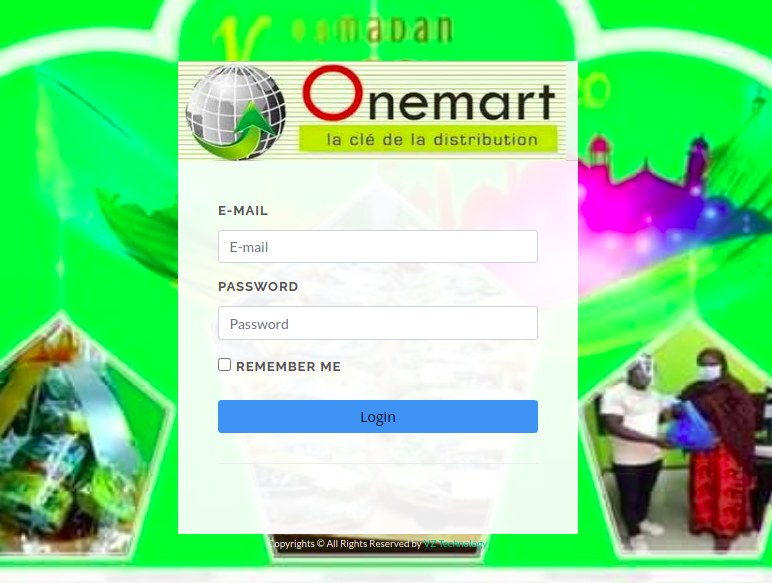
\includegraphics[scale=0.6]{chap_3/authentification.png}
			\captionof{figure}{Page d'authentification}
			\label{page_authentification}
		\end{center}
	\section{Liste des agents}
		Dans cette page on peut voir la liste des agents autorisés à accéder à l'application.
		\begin{center}
			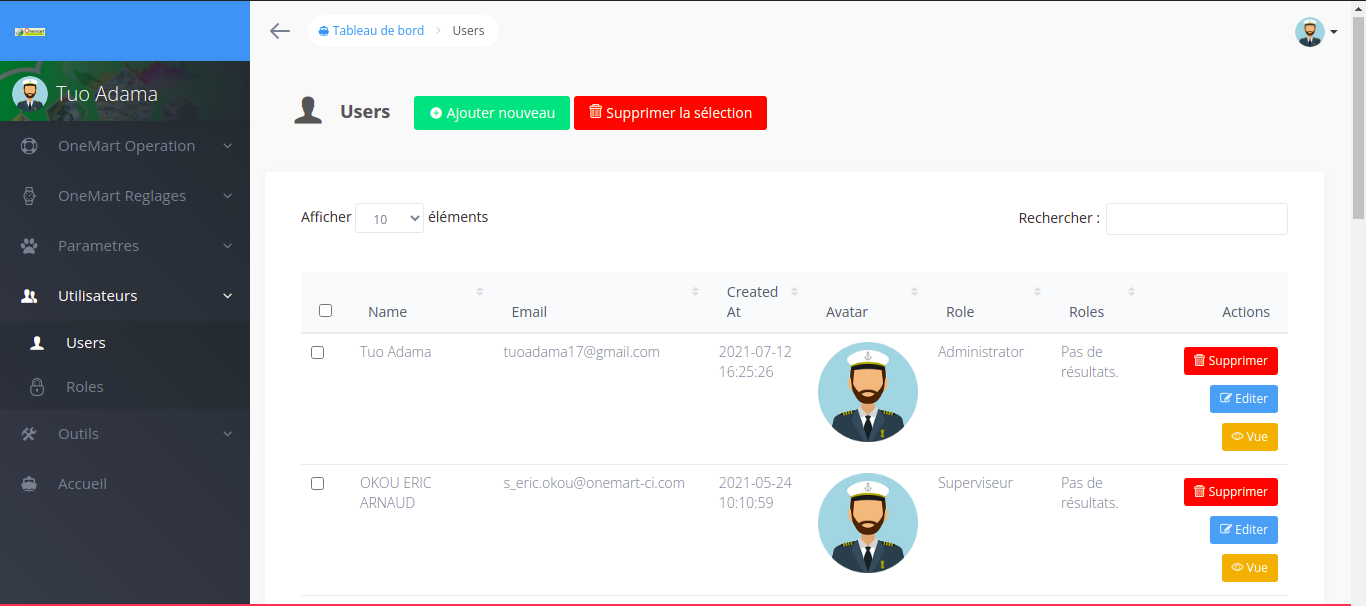
\includegraphics[scale=0.4]{chap_3/utilisateurs.png}
			\captionof{figure}{Liste des agents}
			\label{liste_des_agents}
		\end{center}
	\section{Ajouter d'un agent}
		Page permettant ajouter des agents tout en ayant la possibilité de leurs attribuer des rôles.
		\begin{center}
			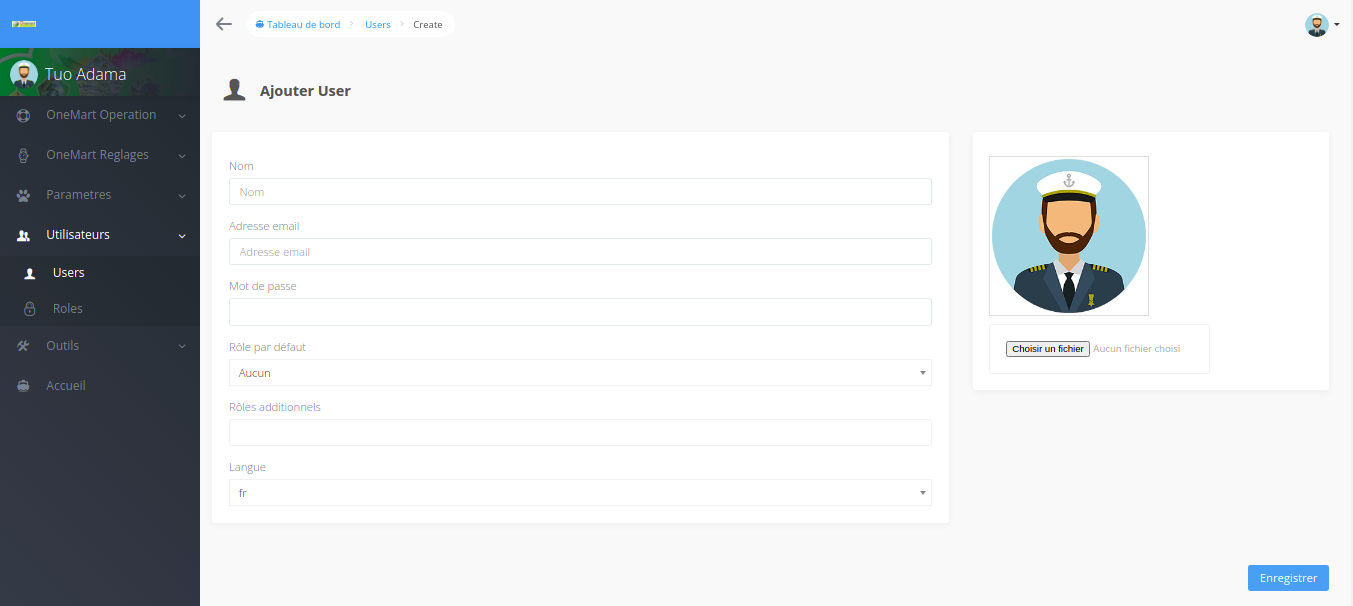
\includegraphics[scale=0.4]{chap_3/ajouter_agent.png}
			\captionof{figure}{Ajouter un agent}
			\label{ajouter_agents}
		\end{center}
	\section{Les Rôles}
		Pour définir une restriction à l'accessibilité aux ressources de l'application, on attribue un ou plusieurs rôle à un utilisateur.
		\begin{center}
			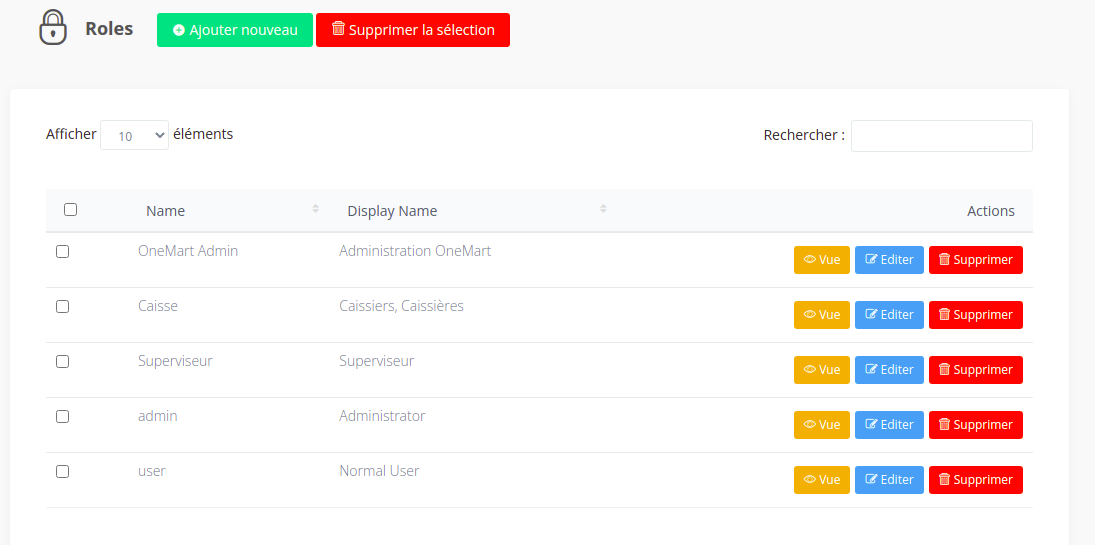
\includegraphics[scale=0.4]{chap_3/roles.png}
			\captionof{figure}{Les rôles}
			\label{les_roles}
		\end{center}
	\section{Ajouter intermède}
		\subsection*{État civil}
		\begin{center}
			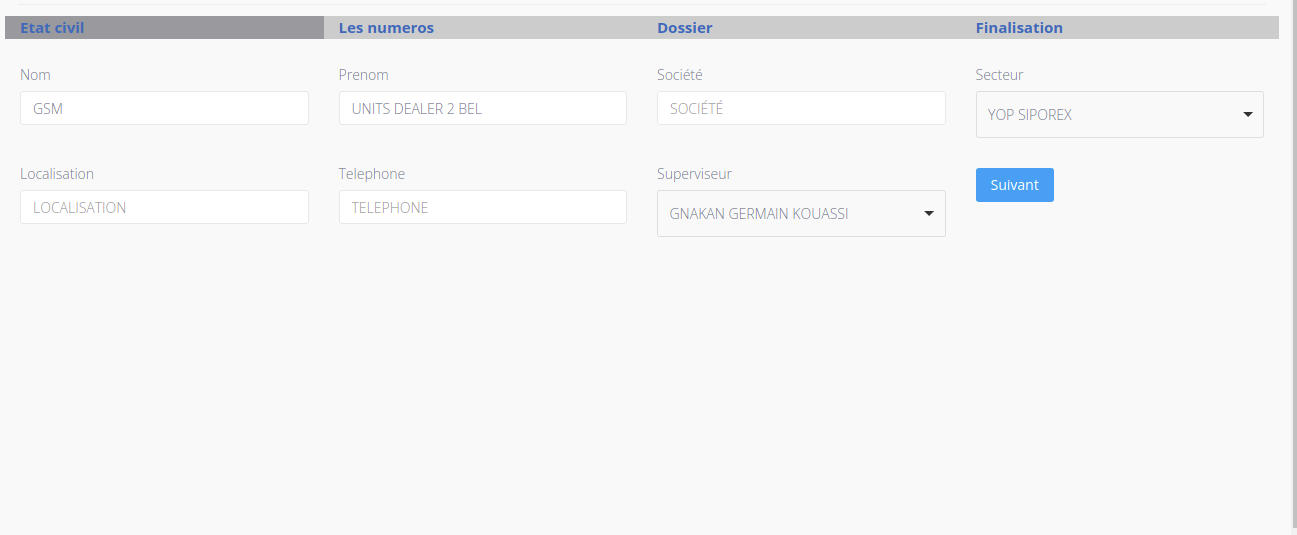
\includegraphics[scale=0.4]{chap_3/ajouter-intermed-etat-civil.png}
			\captionof{figure}{Ajouter intermède}
			\label{ajouter_intermede-etat-civil}
		\end{center}
		\subsection*{Les numéros}
			\begin{center}
				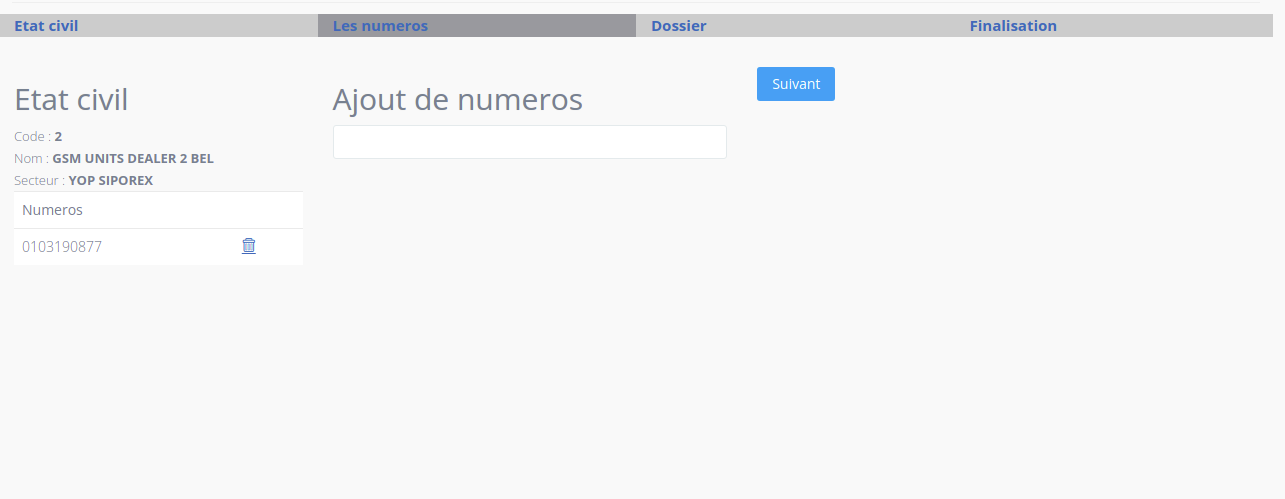
\includegraphics[scale=0.4]{chap_3/ajout-intermed-numeros.png}
				\captionof{figure}{Ajout de numéros}
				\label{ajouter_intermede-les-numeros}
			\end{center}
		
		\subsection*{Photo de profil de l'intermède}
		\begin{center}
			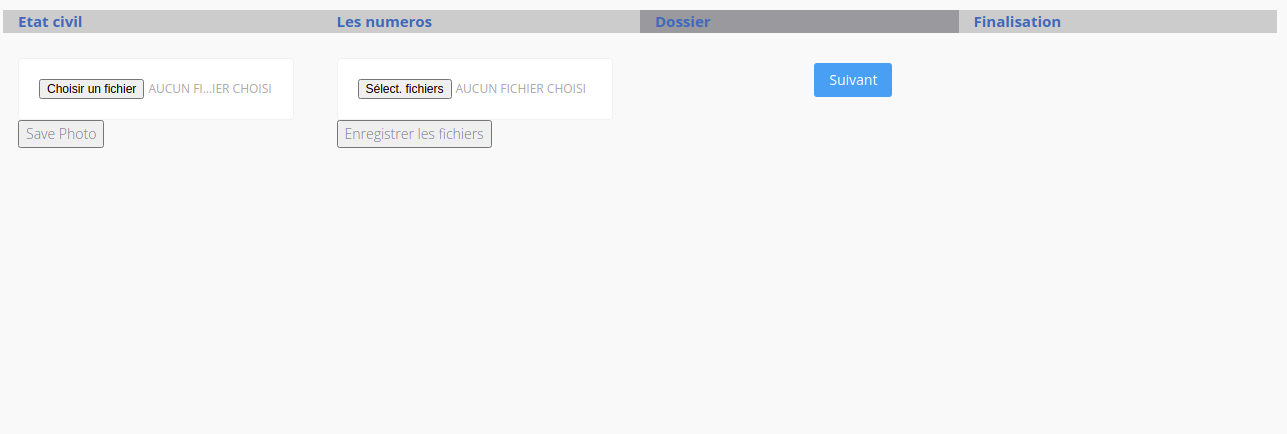
\includegraphics[scale=0.4]{chap_3/ajout-intermed-dossier.png}
			\captionof{figure}{}
			\label{ajouter_intermede-dossier}
		\end{center}
			
	\section{Liste des intermèdes}
		Dans cette on affiche tous les intermèdes avec leur solde.\\
		\begin{center}
			\includegraphics[scale=0.41]{chap_3/liste_intermède.png}
			\captionof{figure}{Liste des intermèdes}
			\label{liste_intermede}
		\end{center}
	\section{Les modes de paiements}
		Cette section concerne les modes de paiements. Nous avons mis en place un système qui pourra s'adapter dans le temps  car elle permettra d'ajouter si on le veut d'autre mode de paiement.\\
		\begin{center}
			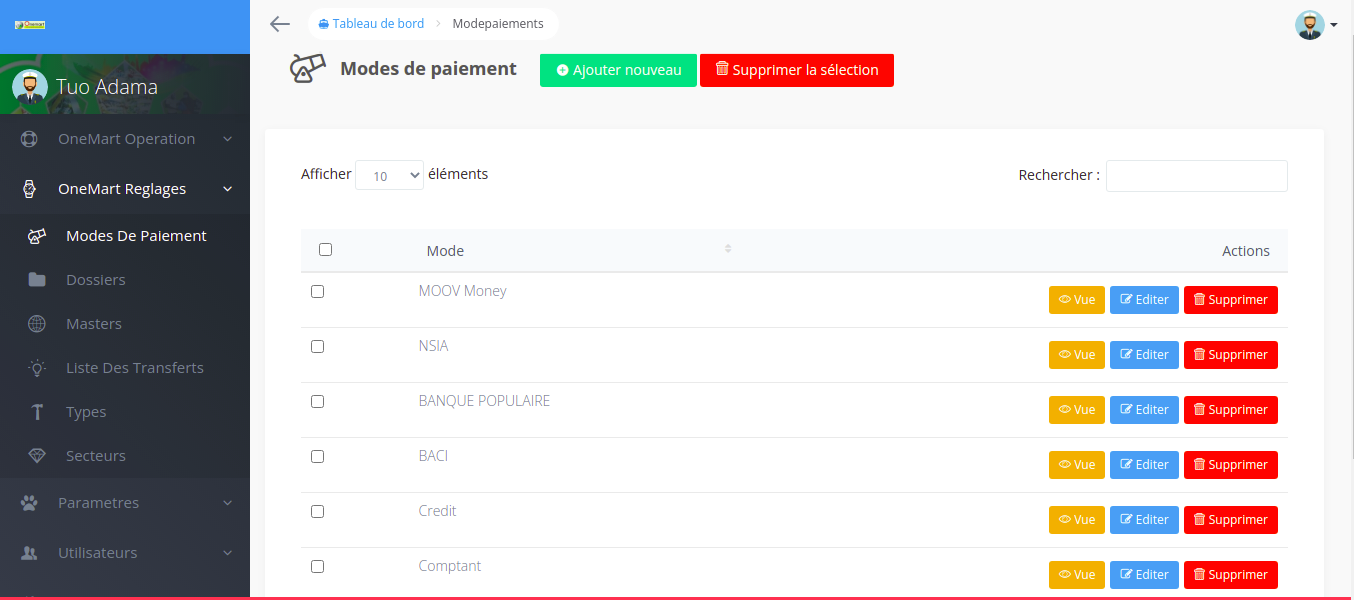
\includegraphics[scale=0.4]{chap_3/mode_paiement.png}
			\captionof{figure}{Mode de paiement}
			\label{mode_de_paiement}
		\end{center}
	\section{Liste des types}
		Dans cette partie également on liste l'ensemble d'opérations que peut effectuer l'agence pour que plus tard on puisse ajouter d'autre nouvelle fonctionnalité.
		\begin{center}
			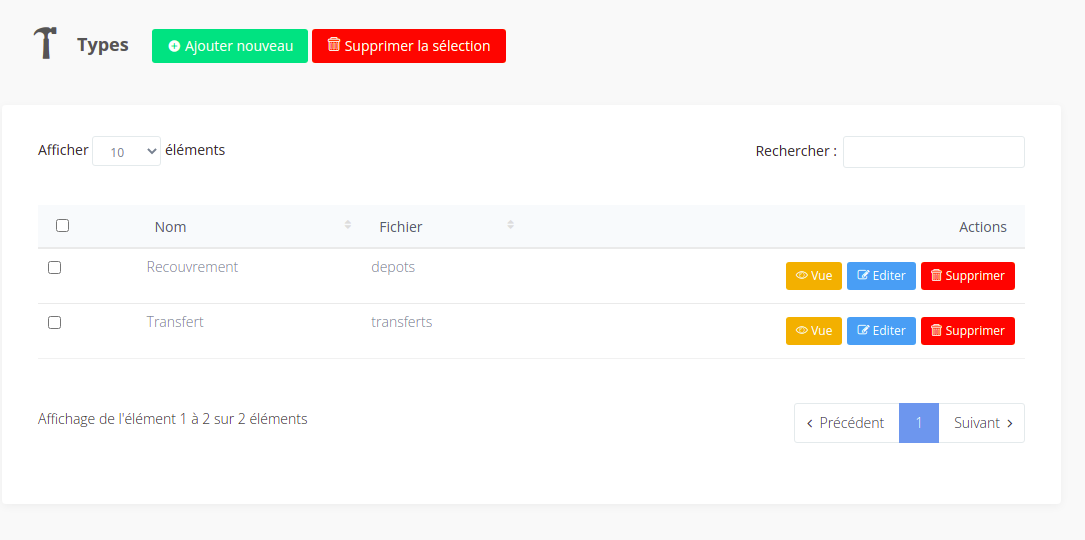
\includegraphics[scale=0.4]{chap_3/types.png}
			\captionof{figure}{Les types}
			\label{mode_de_paiment}
		\end{center}
	\section{Recouvrement}
		Le recouvrement ou encore dépôt se sert des informations présentes sauf que le mode de paiement à crédit n'est pas accessible.\\
		\begin{center}
			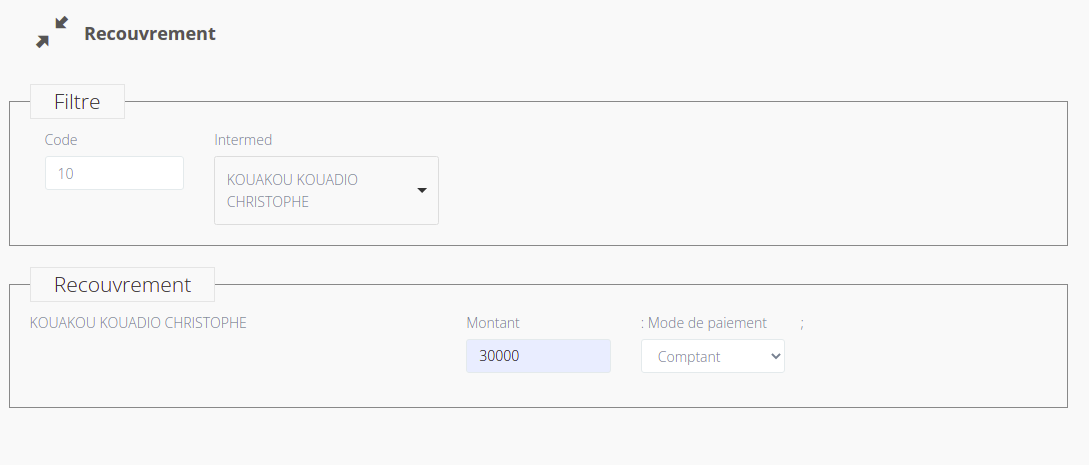
\includegraphics[scale=0.4]{chap_3/recouvrement_1.png}
			\captionof{figure}{Recouvrement}
			\label{recouvrement_1}
		\end{center}
		\begin{center}
			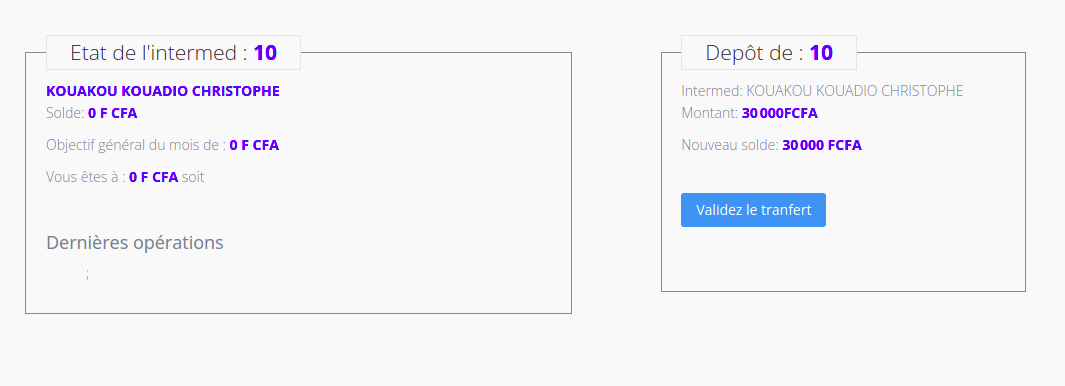
\includegraphics[scale=0.4]{chap_3/recouvrement_2.png}
			\captionof{figure}{Details Recouvrement}
			\label{recouvrement_2}
		\end{center}
		\begin{center}
			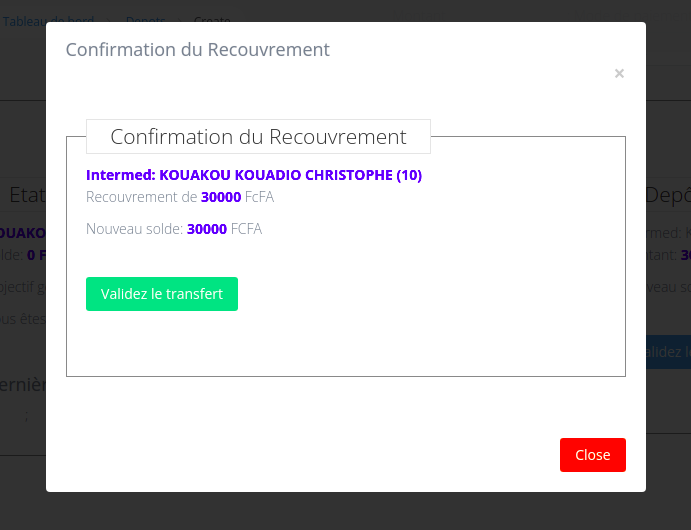
\includegraphics[scale=0.4]{chap_3/recouvrement_3.png}
			\captionof{figure}{Confirmation recouvrement}
			\label{recouvrement_3}
		\end{center}
	\section{Transfert}
		Bien que l'interface de transfert soit similaire à celle du recouvrement, dans le l'opération de transfert on a accès à tous les modes de paiements.
		\begin{center}
			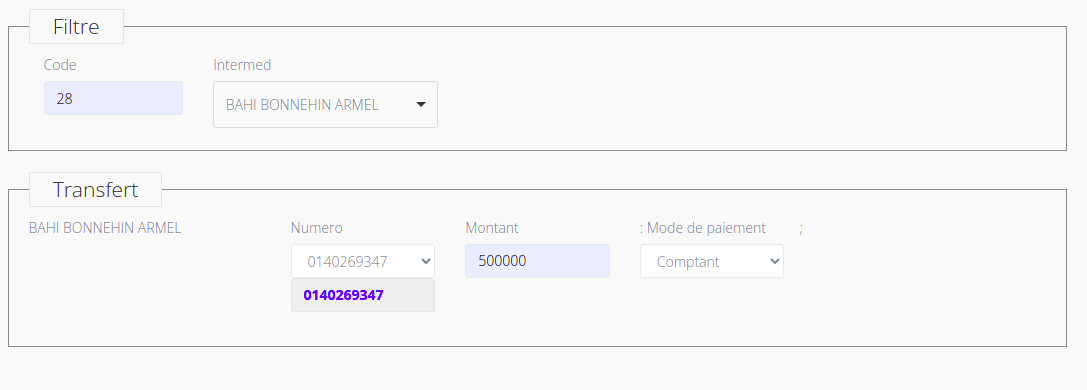
\includegraphics[scale=0.4]{chap_3/transfert_1.png}
			\captionof{figure}{Transfert}
			\label{transfert_1}
		\end{center}
		\begin{center}
			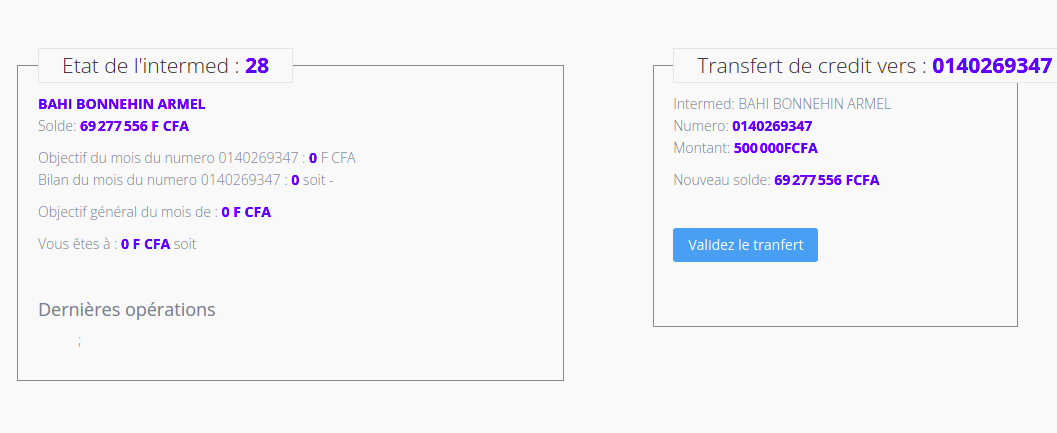
\includegraphics[scale=0.4]{chap_3/transfert_2.png}
			\captionof{figure}{Detail du transfert}
			\label{transfert_2}
		\end{center}
	\section{Facture après une opération}
		Après chaque opération, une facture est délivré à l'intermède. Cette facture se présente comme suite :
		\begin{center}
			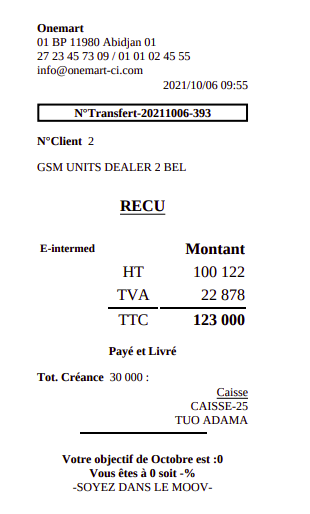
\includegraphics[scale=0.7]{chap_3/facture.png}
			\captionof{figure}{Présentation de facture}
			\label{Facture}
		\end{center}
	\section{Message des opérations}
		Une fois qu'une opération est effectuée, on a un message qui est généré.
		\begin{center}
			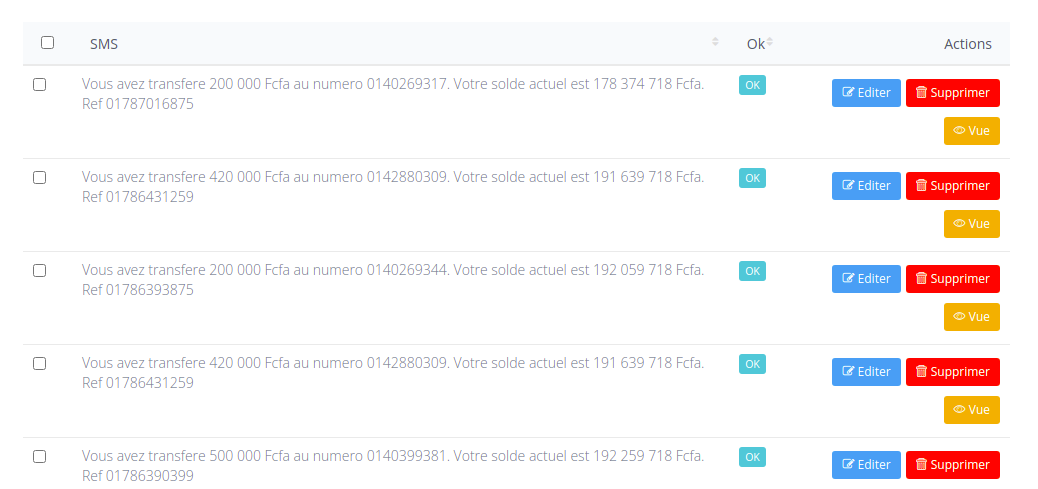
\includegraphics[scale=0.5]{chap_3/message_1.png}
			\captionof{figure}{Message des opérations}
			\label{message}
		\end{center}
		\begin{center}
			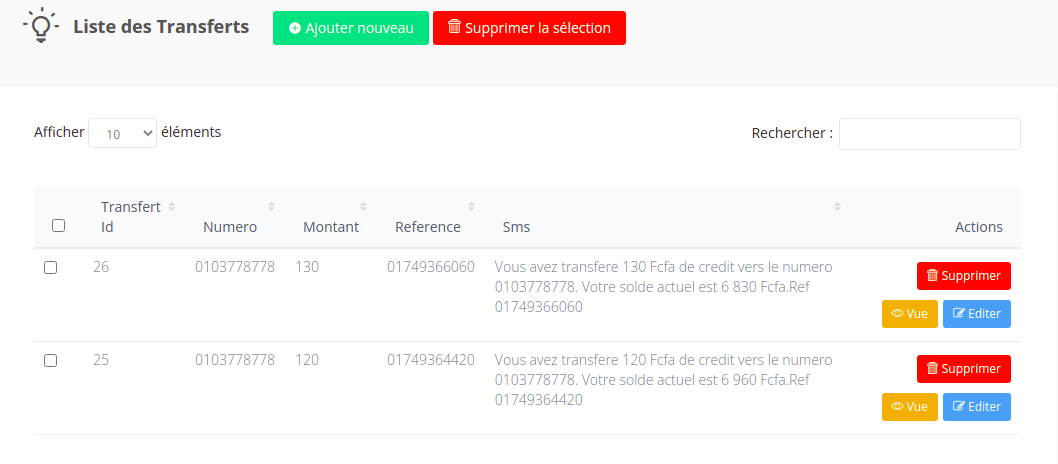
\includegraphics[scale=0.5]{chap_3/message_2.png}
			\captionof{figure}{Message des transferts}
			\label{message_transfert}
		\end{center}
	\section{États des paiements}
		\begin{center}
			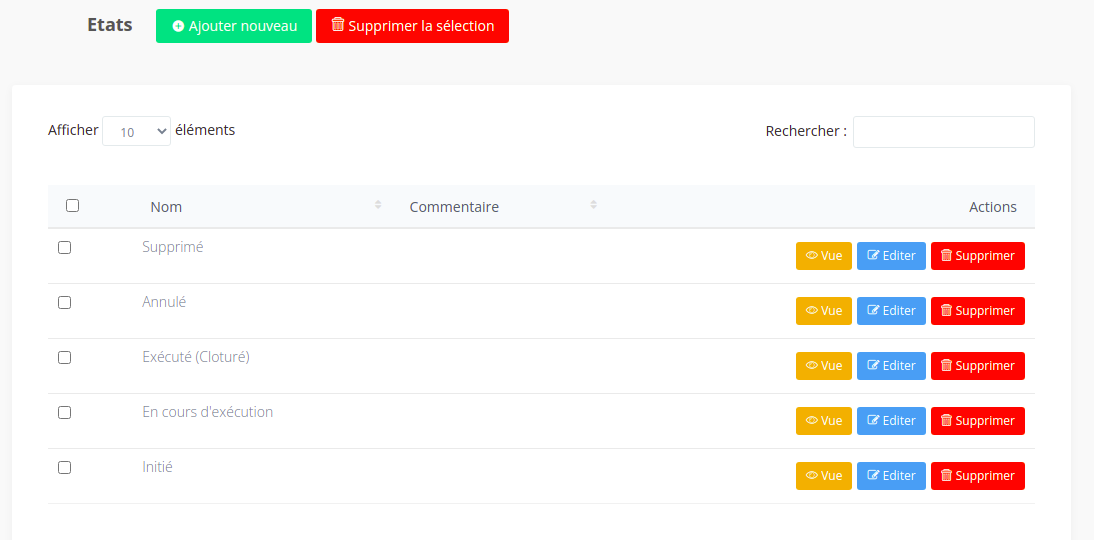
\includegraphics[scale=0.5]{chap_3/etat_de_paiement.png}
			\captionof{figure}{Etat de paiement}
			\label{etat_de_paiement}
		\end{center}
	\section{Conclusion}
		Dans ce chapitre nous avons exploré les grandes parties de notre application grâce aux différentes captures d'écrans et quelque détails pour plus de compréhension.